\documentclass[12pt,a4paper]{article}
\usepackage{tikz}
\usepackage{pgfgantt}

\begin{document}
	\begin{enumerate}
		\item 
			\begin{enumerate}
				\item The following Gantt charts are in the order of FCFS, nonpreemptive SJF, preemptive SJF, nonpreemptive priority, preemptive priority, RR (quantum = $1$), and RR (quantum = $3$).\\
					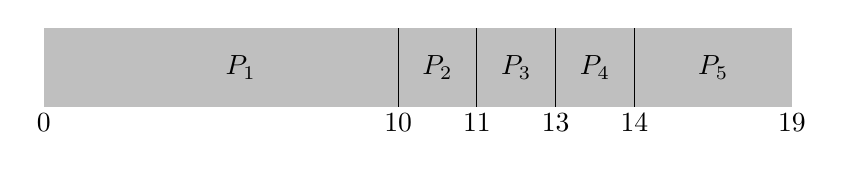
\begin{tikzpicture}
						\fill[gray!50] (0,0) rectangle (9.5,1);
						\draw (4.5,0) -- (4.5,1);
						\draw (5.5,0) -- (5.5,1);
						\draw (6.5,0) -- (6.5,1);
						\draw (7.5,0) -- (7.5,1);
						\tikzstyle{every node}=[];
						\path (2.5,0.5) node (v0) {$P_1$};
						\path (5,0.5) node (v1) {$P_2$};
						\path (6,0.5) node (v2) {$P_3$};
						\path (7,0.5) node (v3) {$P_4$};
						\path (8.5,0.5) node (v4) {$P_5$};
						\path (0,-0.2) node (v5) {$0$};
						\path (4.5,-0.2) node (v6) {$10$};
						\path (5.5,-0.2) node (v7) {$11$};
						\path (6.5,-0.2) node (v8) {$13$};
						\path (7.5,-0.2) node (v9) {$14$};
						\path (9.5,-0.2) node (v10) {$19$};
					\end{tikzpicture}
					
					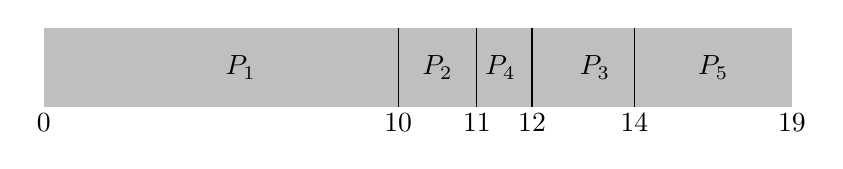
\begin{tikzpicture}
					\fill[gray!50] (0,0) rectangle (9.5,1);
					\draw (4.5,0) -- (4.5,1);
					\draw (5.5,0) -- (5.5,1);
					\draw (6.2,0) -- (6.2,1);
					\draw (7.5,0) -- (7.5,1);
					\tikzstyle{every node}=[];
					\path (2.5,0.5) node (v0) {$P_1$};
					\path (5,0.5) node (v1) {$P_2$};
					\path (5.8,0.5) node (v2) {$P_4$};
					\path (7,0.5) node (v3) {$P_3$};
					\path (8.5,0.5) node (v4) {$P_5$};
					\path (0,-0.2) node (v5) {$0$};
					\path (4.5,-0.2) node (v6) {$10$};
					\path (5.5,-0.2) node (v7) {$11$};
					\path (6.2,-0.2) node (v8) {$12$};
					\path (7.5,-0.2) node (v9) {$14$};
					\path (9.5,-0.2) node (v10) {$19$};
					\end{tikzpicture}
					
					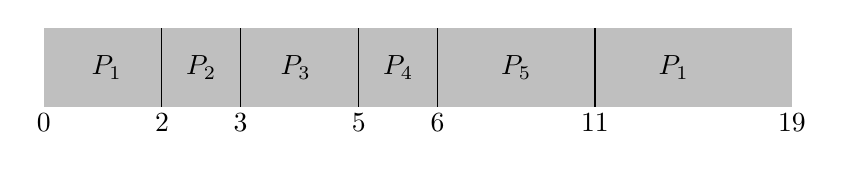
\begin{tikzpicture}
					\fill[gray!50] (0,0) rectangle (9.5,1);
					\draw (1.5,0) -- (1.5,1);
					\draw (2.5,0) -- (2.5,1);
					\draw (4,0) -- (4,1);
					\draw (5,0) -- (5,1);
					\draw (7,0) -- (7,1);
					\tikzstyle{every node}=[];
					\path (0.8,0.5) node (v0) {$P_1$};
					\path (2,0.5) node (v1) {$P_2$};
					\path (3.2,0.5) node (v2) {$P_3$};
					\path (4.5,0.5) node (v3) {$P_4$};
					\path (6.0,0.5) node (v4) {$P_5$};
					\path (8.0,0.5) node (v11) {$P_1$};
					\path (0,-0.2) node (v5) {$0$};
					\path (1.5,-0.2) node (v6) {$2$};
					\path (2.5,-0.2) node (v7) {$3$};
					\path (4,-0.2) node (v8) {$5$};
					\path (5,-0.2) node (v9) {$6$};
					\path (7,-0.2) node (v10) {$11$};
					\path (9.5,-0.2) node (v12) {$19$};
					\end{tikzpicture}
					
					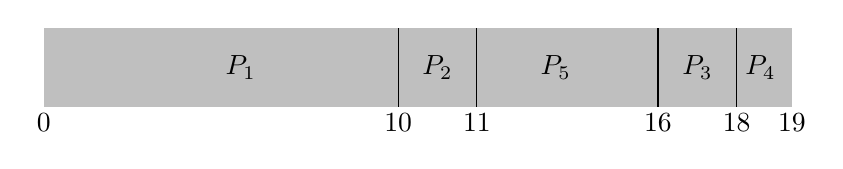
\begin{tikzpicture}
					\fill[gray!50] (0,0) rectangle (9.5,1);
					\draw (4.5,0) -- (4.5,1);
					\draw (5.5,0) -- (5.5,1);
					\draw (7.8,0) -- (7.8,1);
					\draw (8.8,0) -- (8.8,1);
					\tikzstyle{every node}=[];
					\path (2.5,0.5) node (v0) {$P_1$};
					\path (5,0.5) node (v1) {$P_2$};
					\path (6.5,0.5) node (v3) {$P_5$};
					\path (8.3,0.5) node (v4) {$P_3$};
					\path (9.1,0.5) node (v11) {$P_4$};
					\path (0,-0.2) node (v5) {$0$};
					\path (4.5,-0.2) node (v6) {$10$};
					\path (5.5,-0.2) node (v7) {$11$};
					\path (8.8,-0.2) node (v8) {$18$};
					\path (7.8,-0.2) node (v9) {$16$};
					\path (9.5,-0.2) node (v10) {$19$};
					\end{tikzpicture}
					
					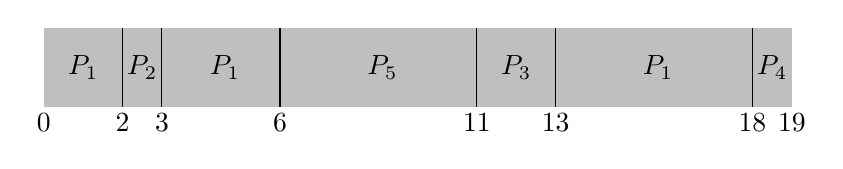
\begin{tikzpicture}
					\fill[gray!50] (0,0) rectangle (9.5,1);
					\draw (1,0) -- (1,1);
					\draw (1.5,0) -- (1.5,1);
					\draw (3,0) -- (3,1);
					\draw (5.5,0) -- (5.5,1);
					\draw (6.5,0) -- (6.5,1);
					\draw (9,0) -- (9,1);
					\tikzstyle{every node}=[];
					\path (0.5,0.5) node (v0) {$P_1$};
					\path (1.25,0.5) node (v1) {$P_2$};
					\path (2.3,0.5) node (v2) {$P_1$};
					\path (4.3,0.5) node (v4) {$P_5$};
					\path (6,0.5) node (v4) {$P_3$};
					\path (7.8,0.5) node (v11) {$P_1$};
					\path (9.25,0.5) node (v16) {$P_4$};
					\path (0,-0.2) node (v5) {$0$};
					\path (1,-0.2) node (v6) {$2$};
					\path (1.5,-0.2) node (v7) {$3$};
					\path (3,-0.2) node (v8) {$6$};
					\path (5.5,-0.2) node (v15) {$11$};
					\path (6.5,-0.2) node (v14) {$13$};
					\path (9,-0.2) node (v13) {$18$};
					\path (9.5,-0.2) node (v12) {$19$};
					\end{tikzpicture}
					
					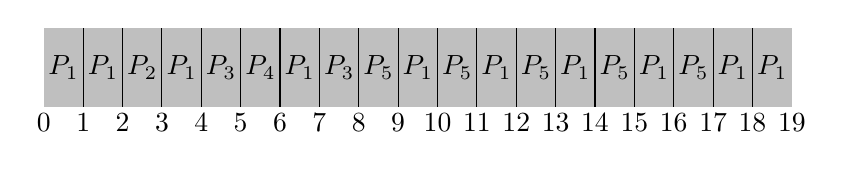
\begin{tikzpicture}
					\fill[gray!50] (0,0) rectangle (9.5,1);
					\draw (0.5,0) -- (0.5,1);
					\draw (1,0) -- (1,1);
					\draw (1.5,0) -- (1.5,1);
					\draw (2,0) -- (2,1);
					\draw (2.5,0) -- (2.5,1);
					\draw (3,0) -- (3,1);
					\draw (3.5,0) -- (3.5,1);
					\draw (4,0) -- (4,1);
					\draw (4.5,0) -- (4.5,1);
					\draw (5,0) -- (5,1);
					\draw (5.5,0) -- (5.5,1);
					\draw (6,0) -- (6,1);
					\draw (6.5,0) -- (6.5,1);
					\draw (7,0) -- (7,1);
					\draw (7.5,0) -- (7.5,1);
					\draw (8,0) -- (8,1);
					\draw (8.5,0) -- (8.5,1);
					\draw (9,0) -- (9,1);
					\tikzstyle{every node}=[];
					\path (0,-0.2) node (v0) {$0$};
					\path (0.5,-0.2) node (v1) {$1$};
					\path (1,-0.2) node (v2) {$2$};
					\path (1.5,-0.2) node (v3) {$3$};
					\path (2.0,-0.2) node (v4) {$4$};
					\path (2.5,-0.2) node (v5) {$5$};
					\path (3.0,-0.2) node (v6) {$6$};
					\path (3.5,-0.2) node (v7) {$7$};
					\path (4.0,-0.2) node (v8) {$8$};
					\path (4.5,-0.2) node (v9) {$9$};
					\path (5.0,-0.2) node (v10) {$10$};
					\path (5.5,-0.2) node (v11) {$11$};
					\path (6.0,-0.2) node (v12) {$12$};
					\path (6.5,-0.2) node (v13) {$13$};
					\path (7.0,-0.2) node (v13) {$14$};
					\path (7.5,-0.2) node (v13) {$15$};
					\path (8.0,-0.2) node (v13) {$16$};
					\path (8.5,-0.2) node (v13) {$17$};
					\path (9.0,-0.2) node (v13) {$18$};
					\path (9.5,-0.2) node (v13) {$19$};
					
					\path (0.25,0.5) node (v0) {$P_1$};
					\path (0.75,0.5) node (v1) {$P_1$};
					\path (1.25,0.5) node (v2) {$P_2$};
					\path (1.75,0.5) node (v3) {$P_1$};
					\path (2.25,0.5) node (v4) {$P_3$};
					\path (2.75,0.5) node (v5) {$P_4$};
					\path (3.25,0.5) node (v6) {$P_1$};
					\path (3.75,0.5) node (v7) {$P_3$};
					\path (4.25,0.5) node (v8) {$P_5$};
					\path (4.75,0.5) node (v9) {$P_1$};
					\path (5.25,0.5) node (v10) {$P_5$};
					\path (5.75,0.5) node (v11) {$P_1$};
					\path (6.25,0.5) node (v12) {$P_5$};
					\path (6.75,0.5) node (v13) {$P_1$};
					\path (7.25,0.5) node (v14) {$P_5$};
					\path (7.75,0.5) node (v15) {$P_1$};
					\path (8.25,0.5) node (v16) {$P_5$};
					\path (8.75,0.5) node (v17) {$P_1$};
					\path (9.25,0.5) node (v18) {$P_1$};
					\end{tikzpicture}
					
					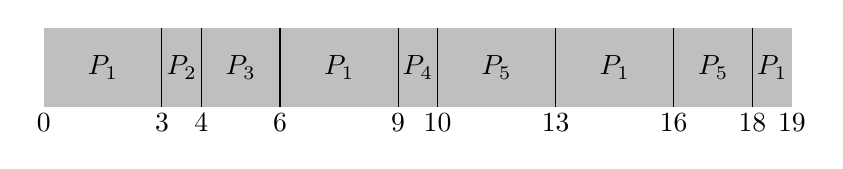
\begin{tikzpicture}
					\fill[gray!50] (0,0) rectangle (9.5,1);
					\draw (1.5,0) -- (1.5,1);
					\draw (2.0,0) -- (2.0,1);
					\draw (3,0) -- (3,1);
					\draw (4.5,0) -- (4.5,1);
					\draw (5,0) -- (5,1);
					\draw (6.5,0) -- (6.5,1);
					\draw (8,0) -- (8,1);
					\draw (9,0) -- (9,1);
					
					\path (0,-0.2) node (v0) {$0$};
					\path (1.5,-0.2) node (v0) {$3$};
					\path (2.0,-0.2) node (v0) {$4$};
					\path (3,-0.2) node (v0) {$6$};
					\path (4.5,-0.2) node (v0) {$9$};
					\path (5,-0.2) node (v0) {$10$};
					\path (6.5,-0.2) node (v0) {$13$};
					\path (8,-0.2) node (v0) {$16$};
					\path (9,-0.2) node (v0) {$18$};
					\path (9.5,-0.2) node (v0) {$19$};
					
					\path (0.75,0.5) node (v18) {$P_1$};
					\path (1.75,0.5) node (v18) {$P_2$};
					\path (2.5,0.5) node (v18) {$P_3$};
					\path (3.75,0.5) node (v18) {$P_1$};
					\path (4.75,0.5) node (v18) {$P_4$};
					\path (5.75,0.5) node (v18) {$P_5$};
					\path (7.25,0.5) node (v18) {$P_1$};
					\path (8.5,0.5) node (v18) {$P_5$};
					\path (9.25,0.5) node (v18) {$P_1$};
					\end{tikzpicture}
					
				\item 
					\begin{itemize}
						\item FCFS: $$\textrm{average waiting time} = \frac{0+8+8+9+8}{5} = 6.6 \textrm{ms}$$
						
						\item nonpreemptive SJF: $$\textrm{average waiting time} = \frac{0+8+7+9+8}{5} = 6.4 \textrm{ms}$$
						
						\item preemptive SJF: $$\textrm{average waiting time} = \frac{9+0+0+1+0}{5} = 2 \textrm{ms}$$
						
						\item nonpreemptive priority: $$\textrm{average waiting time} = \frac{0+8+13+14+5}{5} = 8 \textrm{ms}$$
						
						\item preemptive priority: $$\textrm{average waiting time} = \frac{8+0+8+14+0}{5} = 6 \textrm{ms}$$
						
						\item RR (quantum = $1$): $$\textrm{average waiting time} = \frac{18}{5} = 3.6 \textrm{ms}$$
						
						\item RR (quantum = $3$): $$\textrm{average waiting time} = \frac{23}{5} = 4.6 \textrm{ms}$$
					
					\end{itemize}
				\item 
					\begin{itemize}
						\item FCFS: $$\textrm{average turnaround time} = \frac{10+9+10+10+13}{5} = 10.4 \textrm{ms}$$
						
						\item nonpreemptive SJF: $$\textrm{average turnaround time} = \frac{10+9+8+11+13}{5} = 10.2 \textrm{ms}$$
						
						\item preemptive SJF: $$\textrm{average turnaround time} = \frac{19+1+2+2+5}{5} = 5.8 \textrm{ms}$$
						
						\item nonpreemptive priority: $$\textrm{average turnaround time} = \frac{10+9+15+15+10}{5} = 11.8 \textrm{ms}$$
						
						\item preemptive priority: $$\textrm{average turnaround time} = \frac{18+1+10+15+5}{5} = 9.8 \textrm{ms}$$
						
						\item RR (quantum = $1$): $$\textrm{average turnaround time} = \frac{38}{5} = 7.6 \textrm{ms}$$
						
						\item RR (quantum = $3$): $$\textrm{average turnaround time} = \frac{42}{5} = 8.4 \textrm{ms}$$
						
					\end{itemize}
			\end{enumerate}
		
		\item 
			\begin{enumerate}
				\item 
				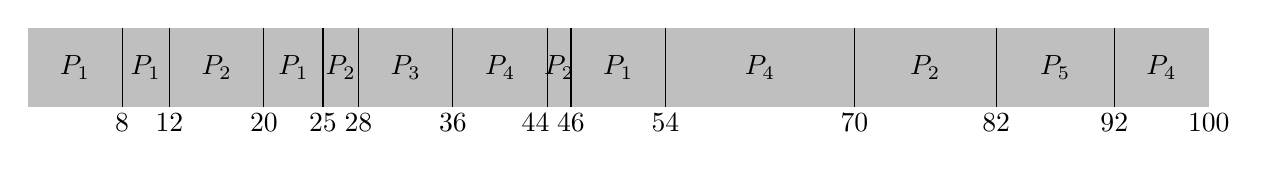
\begin{tikzpicture}
				\fill[gray!50] (0,0) rectangle (15,1);
				\draw (0.8*1.5,0) -- (0.8*1.5,1);
				\draw (1.2*1.5,0) -- (1.2*1.5,1);
				\draw (2.0*1.5,0) -- (2.0*1.5,1);
				\draw (2.5*1.5,0) -- (2.5*1.5,1);
				\draw (2.8*1.5,0) -- (2.8*1.5,1);
				\draw (3.6*1.5,0) -- (3.6*1.5,1);
				\draw (4.4*1.5,0) -- (4.4*1.5,1);
				\draw (4.6*1.5,0) -- (4.6*1.5,1);
				\draw (5.4*1.5,0) -- (5.4*1.5,1);
				\draw (7.0*1.5,0) -- (7.0*1.5,1);
				\draw (8.2*1.5,0) -- (8.2*1.5,1);
				\draw (9.2*1.5,0) -- (9.2*1.5,1);
				
				\path (0.8*1.5,-0.2) node (v0) {$8$};
				\path (1.2*1.5,-0.2) node (v0) {$12$};
				\path (2*1.5,-0.2) node (v0) {$20$};
				\path (2.5*1.5,-0.2) node (v0) {$25$};
				\path (2.8*1.5,-0.2) node (v0) {$28$};
				\path (3.6*1.5,-0.2) node (v0) {$36$};
				\path (4.3*1.5,-0.2) node (v0) {$44$};
				\path (4.6*1.5,-0.2) node (v0) {$46$};
				\path (5.4*1.5,-0.2) node (v0) {$54$};
				\path (7*1.5,-0.2) node (v0) {$70$};
				\path (8.2*1.5,-0.2) node (v0) {$82$};
				\path (9.2*1.5,-0.2) node (v0) {$92$};
				\path (10*1.5,-0.2) node (v0) {$100$};
				
				\path (0.4*1.5,0.5) node (v18) {$P_1$};
				\path (1*1.5,0.5) node (v18) {$P_1$};
				\path (1.6*1.5,0.5) node (v18) {$P_2$};
				\path (2.25*1.5,0.5) node (v18) {$P_1$};
				\path (2.65*1.5,0.5) node (v18) {$P_2$};
				\path (3.2*1.5,0.5) node (v18) {$P_3$};
				\path (4.0*1.5,0.5) node (v18) {$P_4$};
				\path (4.5*1.5,0.5) node (v18) {$P_2$};
				\path (5*1.5,0.5) node (v18) {$P_1$};
				\path (6.2*1.5,0.5) node (v18) {$P_4$};
				\path (7.6*1.5,0.5) node (v18) {$P_2$};
				\path (8.7*1.5,0.5) node (v18) {$P_5$};
				\path (9.6*1.5,0.5) node (v18) {$P_4$};
				\end{tikzpicture}
				
				\item There are 12 context switches for the processes.
				
				\item The average waiting time is $(8+45+0+32+28)/5=22.6$ ms. The average turnaround time is $(8+64+25+70+46)/5=42.6$ ms.
			\end{enumerate}
		\item
		\begin{itemize}
			\item[(1)] If the Shortest job first algorithm is preemptive, then it could result in starvation if the currently executing process has a pretty long CPU burst and there are lots of processes with shorter CPU burst entering the ready queue, the currently executing process would be preempted and may suffer from starvation.
			
			\item[(2)] Priority Scheduling algorithm may also result in starvation, since a
			steady stream of higher-priority processes can prevent a low-priority process
			from ever getting the CPU.
		\end{itemize} 
		
	\end{enumerate}
\end{document}
